\begin{frame}
  \begin{figure}
    \centering
    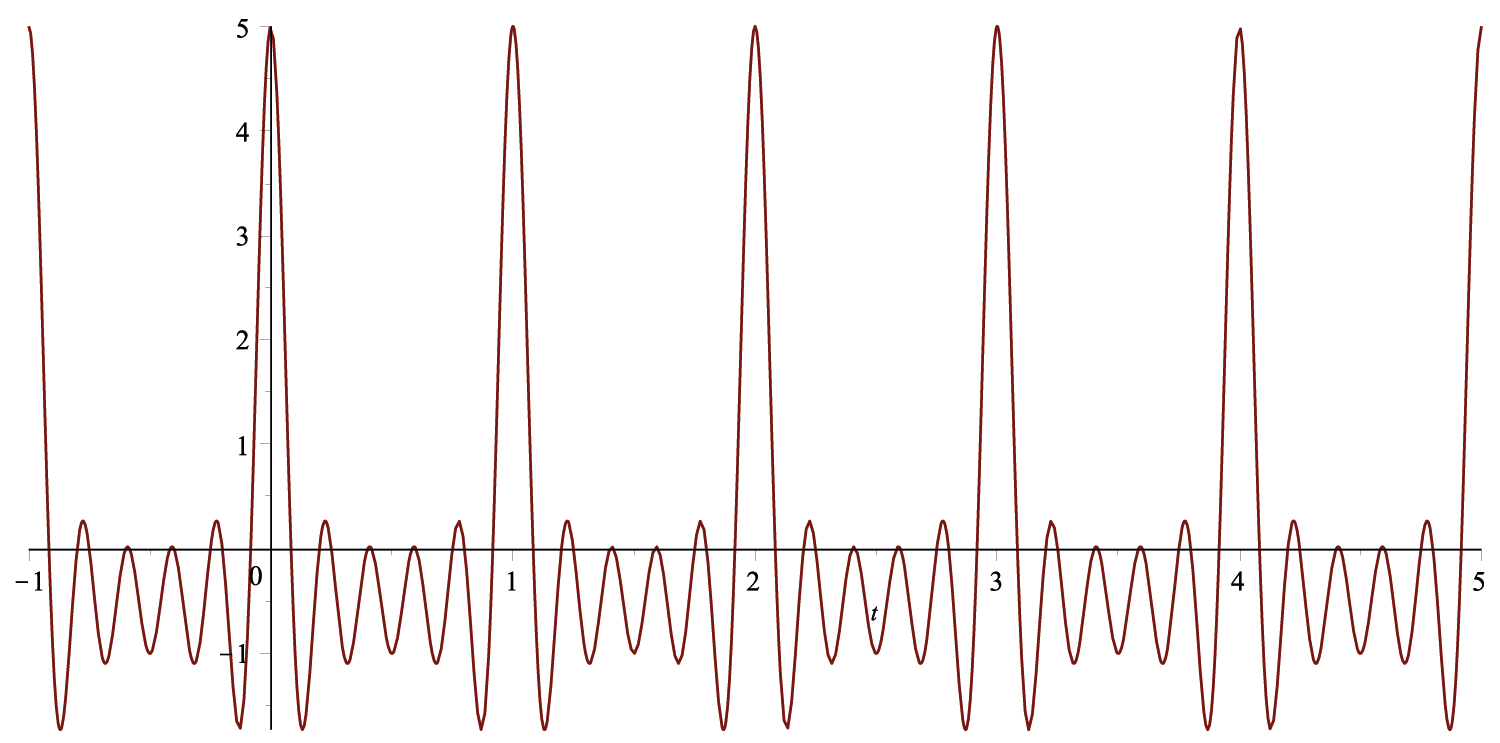
\includegraphics[width=\linewidth]{img/intro_harmonics}
    \caption{Auslenkungs-Zeit-Diagramm von Grund- und Oberschwingungen}
    \label{img:harmonics}
  \end{figure}
\end{frame}

\begin{frame}
  \begin{figure}
    \centering
    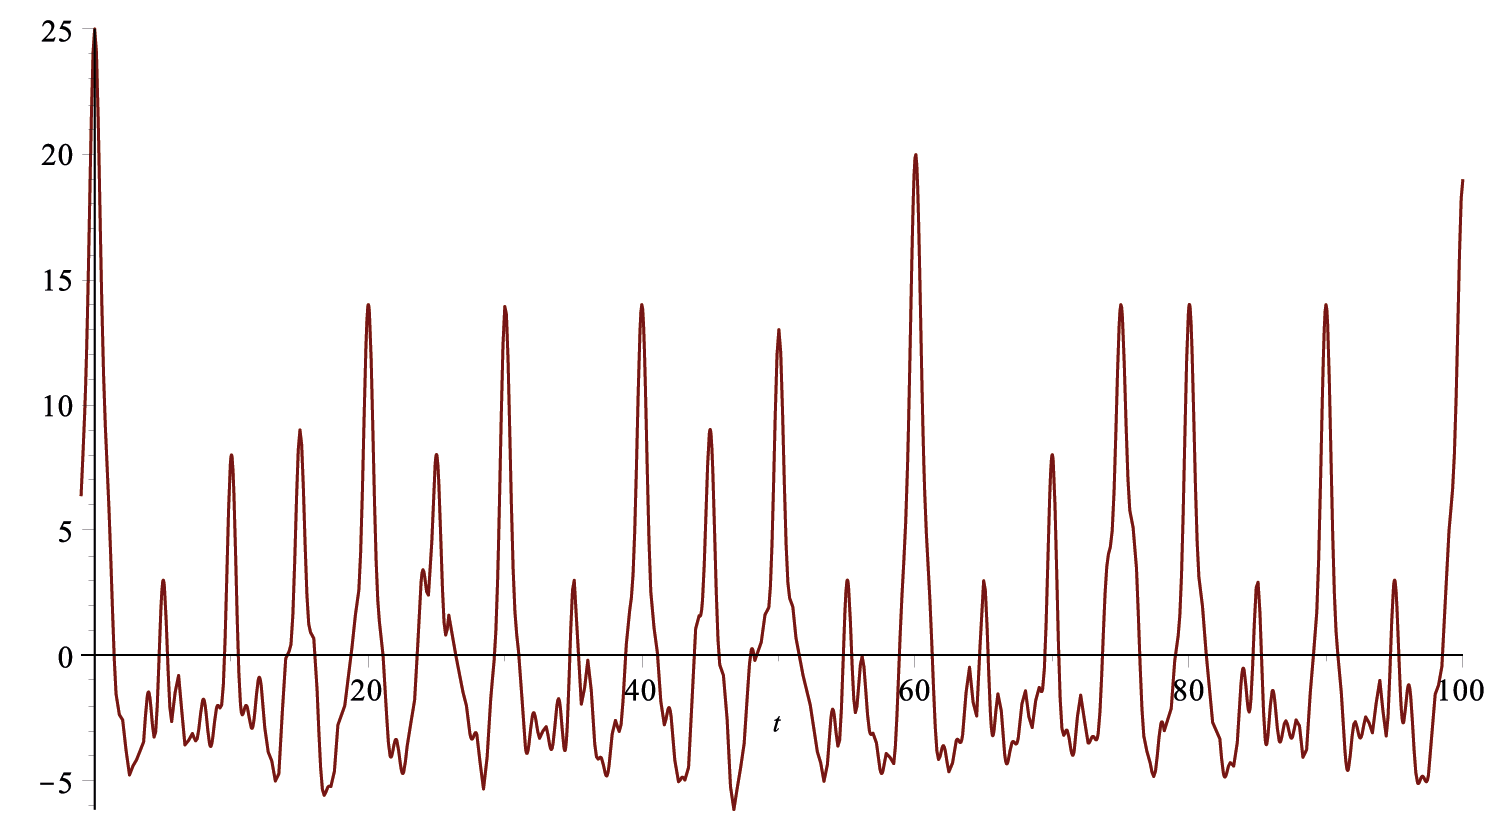
\includegraphics[width=\linewidth]{img/intro_interference}
    \caption{Auslenkungs-Zeit-Diagramm von verschiedenen Grund- und Oberschwingungen}
    \label{img:interference}
  \end{figure}
\end{frame}
